\documentclass{article}



\usepackage{arxiv}

\usepackage[utf8]{inputenc} % allow utf-8 input
\usepackage[T1]{fontenc}    % use 8-bit T1 fonts
\usepackage{hyperref}       % hyperlinks
\usepackage{url}            % simple URL typesetting
\usepackage{booktabs}       % professional-quality tables
\usepackage{amsfonts}       % blackboard math symbols
\usepackage{nicefrac}       % compact symbols for 1/2, etc.
\usepackage{microtype}      % microtypography
\usepackage{lipsum}   % Can be removed after putting your text content
\usepackage{graphicx}
\usepackage{natbib}
\usepackage{doi}

\newcommand{\insertPdfFig}[3]{
  \begin{figure}[h]
  \centering
  \includegraphics[width=16.4cm]{#1.pdf}
  \caption{#2}
  \label{fig:#1}
  \end{figure}
}

\newcommand{\insertSmallPdfFig}[3]{
  \begin{figure}[h]
  \centering
  \includegraphics[width=8.4cm]{#1.pdf}
  \caption{#2}
  \label{fig:#1}
  \end{figure}
}

\title{Detecting Outliers in Mortality Data using Cross-Validated Confidence Intervals}
\graphicspath{{../../figures/paper}}
%\date{September 9, 1985} % Here you can change the date presented in the paper title
%\date{}          % Or removing it

\author{Matz A. Haugen \\
\texttt{matzhaugen@gmail.com} \\
  \And
  Dorothea Gilbert \\
  %% \AND
  %% Coauthor \\
  %% Affiliation \\
  %% Address \\
  %% \texttt{email} \\
  %% \And
  %% Coauthor \\
  %% Affiliation \\
  %% Address \\
  %% \texttt{email} \\
  %% \And
  %% Coauthor \\
  %% Affiliation \\
  %% Address \\
  %% \texttt{email} \\
}

% Uncomment to remove the date
%\date{}

% Uncomment to override  the `A preprint' in the header
%\renewcommand{\headeright}{Technical Report}
%\renewcommand{\undertitle}{Technical Report}
\renewcommand{\shorttitle}{Detecting Outliers in Mortality Data}

%%% Add PDF metadata to help others organize their library
%%% Once the PDF is generated, you can check the metadata with
%%% $ pdfinfo template.pdf
\hypersetup{
pdftitle={A template for the arxiv style},
pdfsubject={q-bio.NC, q-bio.QM},
pdfauthor={Matz A. Haugen},
pdfkeywords={Mortality, Outliers, Splines, Confidence intervals},
}

\begin{document}
\maketitle

\begin{abstract}
  \lipsum[1]
\end{abstract}


% keywords can be removed
\keywords{Mortality \and Outliers}


\section{Introduction}
\lipsum[2]

\section{Methods}
\label{sec:methods}

\section{Results}
\label{sec:results}


\insertPdfFig{population_rates}{Population in Norway 2001-2022. Data is collected annually at the end of each year and interpolated to a weekly resolution.}

\insertPdfFig{weekly_deaths_variance}{Weekly means and variance for mortality data from 2001-2022, separated into age-brackets of 5 years.}

\insertSmallPdfFig{norway_gompertz_law_ln_mortality_rates}{Gompertz law of mortality in Norway: Log-transformed death rates plotted against age using a 5-year age bracket. The average age is taken as the observation on the abscissa. A linear trend is fitted with a weighted squared error loss after age 30 and a natural spline with 4 degrees of freedom before age 30.}


\insertPdfFig{norway_mortality_rates}{Mortality rates separated into age brackets. Top: Natural-Log-transformed mortality rates. Bottom: Raw mortality rates. Units are different in the y-axis due to the transformation. This is to show both the linear rise in mortality with age and the corresponding change in temporal variance. Notice on the top how variance is lowest in the middle ages.}


\insertPdfFig{norway_ln_mort_rate_2001_2021}{Log-transformed mortality rate for people over 65 years in Norway after age-standardization, using annual population in 5-year age brackets. A trend is added with two splines one for decadal trends (4 degrees of freedom) and one for seasonal trends (7 degrees of freedom). A constant trend is assumed in the years 2020-2021.}


\insertPdfFig{detrended_mortality}{Histogram of weekly deaths for ages above 65 in Norway, juxtaposed with a Poisson distribution with a mean/variance of 500
.}

\insertPdfFig{norway_excess_deaths_pois}{Excess deaths for people over 65 years in Norway after age-standardization and detrending with a seasonal and decadal trend. Trends are fitted robustly at the $50^{th}$ quantile, while the confidence interval fits the 97.5\% and the 2.5\% quantiles respectively. Vaccination data is superimposed for the same age group, separated by injection number.}


\insertPdfFig{cv_pois_s2008}{Cross-Validated Exceedence Estimates: An estimate of the exceedence fraction of annual observations from 2001-2019 outside the $95^{th}$ confidence band for the training period (blue) and for the out-of-sample hold-out year (in red). Each year is held out in turn while the other years are used to compute the confidence band. Error bars are one standard deviation of the average estimate.}


% \begin{figure}
%   \centering
%   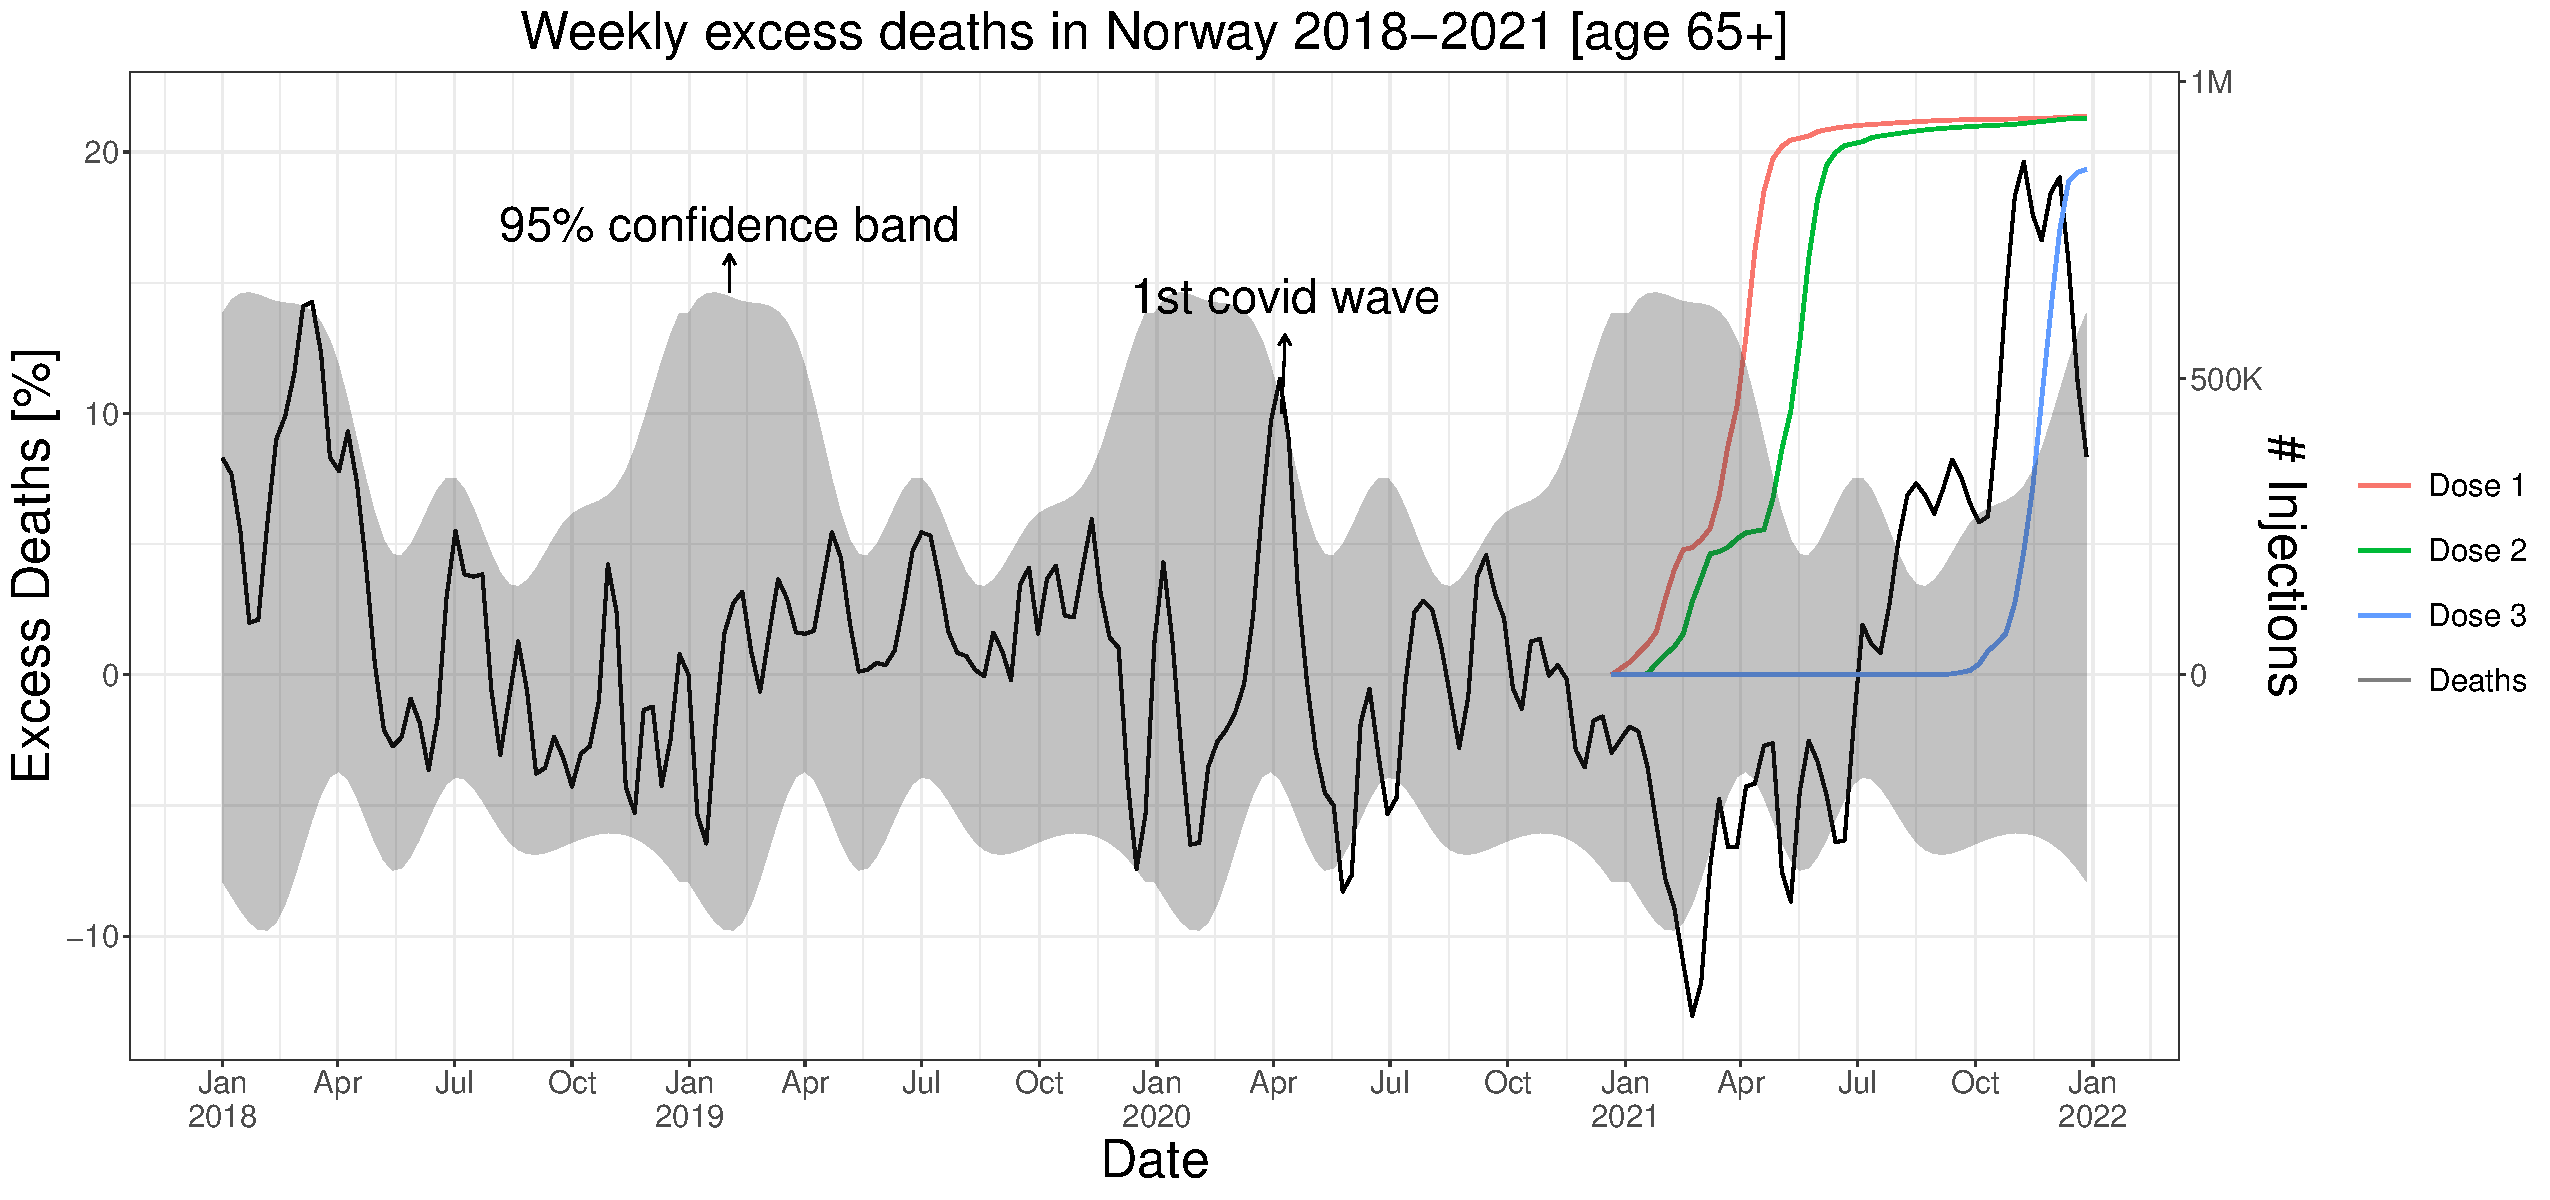
\includegraphics[width=17.4cm]{norway_excess_deaths_pois.pdf}
%   \caption{This caption would be placed at the side of the figure, rather than below it.}
%   \label{fig:fig1}
% \end{figure}

% \subsection{Tables}
% See awesome Table~\ref{tab:table}.

% The documentation for \verb+booktabs+ (`Publication quality tables in LaTeX') is available from:
% \begin{center}
%   \url{https://www.ctan.org/pkg/booktabs}
% \end{center}


% \begin{table}
%   \caption{Sample table title}
%   \centering
%   \begin{tabular}{lll}
%     \toprule
%     \multicolumn{2}{c}{Part}                   \\
%     \cmidrule(r){1-2}
%     Name     & Description     & Size ($\mu$m) \\
%     \midrule
%     Dendrite & Input terminal  & $\sim$100     \\
%     Axon     & Output terminal & $\sim$10      \\
%     Soma     & Cell body       & up to $10^6$  \\
%     \bottomrule
%   \end{tabular}
%   \label{tab:table}
% \end{table}

\bibliographystyle{unsrtnat}

\bibliography{../references}  %%% Uncomment this line and comment out the ``thebibliography'' section below to use the external .bib file (using bibtex) .


%%% Uncomment this section and comment out the \bibliography{references} line above to use inline references.
% \begin{thebibliography}{1}

%   \bibitem{kour2014real}
%   George Kour and Raid Saabne.
%   \newblock Real-time segmentation of on-line handwritten arabic script.
%   \newblock In {\em Frontiers in Handwriting Recognition (ICFHR), 2014 14th
%       International Conference on}, pages 417--422. IEEE, 2014.

%   \bibitem{kour2014fast}
%   George Kour and Raid Saabne.
%   \newblock Fast classification of handwritten on-line arabic characters.
%   \newblock In {\em Soft Computing and Pattern Recognition (SoCPaR), 2014 6th
%       International Conference of}, pages 312--318. IEEE, 2014.

%   \bibitem{hadash2018estimate}
%   Guy Hadash, Einat Kermany, Boaz Carmeli, Ofer Lavi, George Kour, and Alon
%   Jacovi.
%   \newblock Estimate and replace: A novel approach to integrating deep neural
%   networks with existing applications.
%   \newblock {\em arXiv preprint arXiv:1804.09028}, 2018.

% \end{thebibliography}


\end{document}